\documentclass[12pt]{article}
\usepackage{makeidx}
\usepackage[margin=1in]{geometry}  % set the margins to 1in on all sides
\usepackage{graphicx}              % to include figures
\usepackage{amsmath}               % great math stuff
\usepackage{amsfonts}              % for blackboard bold, etc
\usepackage{amsthm}                % better theorem environments
\usepackage{makeidx}               % index
\usepackage[utf8]{inputenc}        % now we have tildes!
\usepackage{wrapfig}               % images
\usepackage{listings}              % Unordered lists

% various theorems, numbered by section

\makeindex



\newtheorem{thm}{Theorem}[section]
\newtheorem{lem}[thm]{Lemma}
\newtheorem{prop}[thm]{Proposition}
\newtheorem{cor}[thm]{Corollary}
\newtheorem{conj}[thm]{Conjecture}

\graphicspath{{maps/}}

\lstset{numberstyle=\scriptsize\ttfamily, numbersep=7pt, captionpos=b}
\lstset{basicstyle=\small\ttfamily}
\lstset{framesep=2pt}

\DeclareMathOperator{\id}{id}

\newcommand{\bd}[1]{\mathbf{#1}}  % for bolding symbols
\newcommand{\RR}{\mathbb{R}}      % for Real numbers
\newcommand{\ZZ}{\mathbb{Z}}      % for Integers
\newcommand{\col}[1]{\left[\begin{matrix} #1 \end{matrix} \right]}
\newcommand{\comb}[2]{\binom{#1^2 + #2^2}{#1+#2}}

\begin{document}

\begin{titlepage}

\newcommand{\HRule}{\rule{\linewidth}{0.5mm}} % Defines a new command for the horizontal lines, change thickness here

\center % Center everything on the page

%----------------------------------------------------------------------------------------
%	HEADING SECTIONS
%----------------------------------------------------------------------------------------

\textsc{\LARGE Universidad Carlos III de Madrid}\\[1.5cm] % Name of your university/college
\textsc{\Large Aprendizaje Automático}\\[0.5cm] % Major heading such as course name
\textsc{\large Computer Science Engineering}\\[0.5cm] % Minor heading such as course title

%----------------------------------------------------------------------------------------
%	TITLE SECTION
%----------------------------------------------------------------------------------------

\HRule \\[0.4cm]
{ \huge \bfseries Tutorial 1: Plataforma PacMan}\\[0.4cm] % Title of your document
\HRule \\[1.5cm]

%----------------------------------------------------------------------------------------
%	AUTHOR SECTION
%----------------------------------------------------------------------------------------


% If you don't want a supervisor, uncomment the two lines below and remove the section above
\emph{Authors:}\\
Daniel \textsc{Medina García}\\ % Your name
Alejandro \textsc{Rodríguez Salamanca}\\[3cm] % Your name

%----------------------------------------------------------------------------------------
%	DATE SECTION
%----------------------------------------------------------------------------------------

{\large \today}\\[3cm] % Date, change the \today to a set date if you want to be precise

%----------------------------------------------------------------------------------------
%	LOGO SECTION
%----------------------------------------------------------------------------------------

%
\includegraphics{Logo}\\[1cm] % Include a department/university logo - this will require the graphicx package

%----------------------------------------------------------------------------------------

\vfill % Fill the rest of the page with whitespace

\end{titlepage}

\tableofcontents

\newpage

\begin{center}
\section{Preguntas:}

\subsection{Pregunta 1}

\emph{¿Qué información se muestra en la interfaz? ¿Y en la terminal? ¿Cuál es la
posición que ocupa PacMan inicialmente?}\\
\end{center}

En la interfaz se muestra el tablero con PacMan. En la parte inferior podemos
observar los indicadores de qué fantasmas han sido comidos, así como la
puntuación de la partida y cuatro números, cada uno del color de un fantasma,
que se corresponden con la distancia que hay desde PacMan a los fantasmas

En la terminal no se muestra ninguna información.

La posición que ocupa PacMan al inicio de la partida depende del mapa usado. En
ciertos mapas, PacMan se encuentra en la esquina superior izquierda, en otros,
PacMan sale en la fila interior, centrado.


\newpage
\begin{center}
\subsection{Pregunta 2}

\emph{Según tu opinión, ¿qué datos podrían ser útiles para decidir lo que tiene
que hacer PacMan en cada momento?}\\
\end{center}

Los datos que podrían interesarnos para decidir qué dirección debe tomar
PacMan son:

\begin{itemize}
    \item \textbf{Distancia de PacMan a los fantasmas}: sabiendo la distancia
    que hay de PacMan a los fantasmas, podremos decidir en cada turno qué
    objetivo es el más cercano. Dado que en algunos mapas existen paredes que
    PacMan no puede atravesar, habría que encontrar una función que tuviese
    esto en cuenta a la hora de calcular la distancia, ya que puede que PacMan
    y un fantasma se encuentren a una distancia de dos casillas en el mapa,
    pero entre medias exista una pared, por lo que la distancia real sería mayor.
    \item \textbf{Dirección en la que se encuentran los fantasmas}: Si PacMan
    sabe en qué dirección se encuentran los fantasmas, podría dirigirse
    directamente en esa dirección. La distancia únicamente, no ayudaría a
    PacMan a decidir qué dirección tomar.
    \item \textbf{Densidad de fantasmas en una zona}: Con este parámetro,
    podríamos saber si en cierta zona del mapa se encuentran más fantasmas, y
    tomar la decisión de dirigirnos hacia esa zona en vez de hacia otra zona en
    la que solo se encuentre un fantasma, pese a que éste se encuentre a una
    distancia menor, ya que existiría la posibilidad de eliminar más fantasmas.
    \item \textbf{Posición y dirección de PacMan}: si conocemos la posición
    actual de PacMan y la posición en la que se está moviendo, podremos decidir
    mejor a por qué fantasmas nos conviene ir. Por ejemplo, si PacMan se está
    moviendo hacia la derecha y uno de los fantasmas se mueve hacia la
    izquierda, PacMan llegará hasta él antes que hasta otro fantasma que esté a
    priori más cerca, pero se esté moviendo en la misma dirección.
\end{itemize}


\newpage
\begin{center}
\subsection{Pregunta 3}

\emph{Revisa la carpeta layouts. ¿Cómo están definidos los mapas en estos
ficheros? Diseña un mapa nuevo, guárdalo y ejecútalo en el juego.}
\end{center}

Están definidos por caracteres en archivos de texto con la extensión .lay.
 Cada carácter representa una casilla en el mapa.

\begin{itemize}
    \item \textbf{\% - Paredes}. Son casillas que PacMan no puede atravesar
    \item \textbf{G} - Representa la posición inicial de los fantasmas.
    \item \textbf{P} - Representa la posición inicial de PacMan.
    \item \textbf{.} - Casilla que PacMan puede comer. En esta implementación
    estas casillas no son tenidas en cuenta.
    \item \textbf{o} - Casilla que PacMan puede comer. En esta implementación
    estas casillas no son tenidas en cuenta.
    \item Además, si el formato de la penúltima fila del mapa es del tipo \% \%
    \% \% \% \% \%\%\%\%\%\%\%\%\%\%\%\%\%\%\%\%\%\%, en el juego se verá qué
    fantasmas han sido comidos por PacMan en la parte inferior del mapa.
\end{itemize}

El nuevo mapa creado por nosotros es el siguiente:\\
\begin{center}
    \vspace{-17pt}
    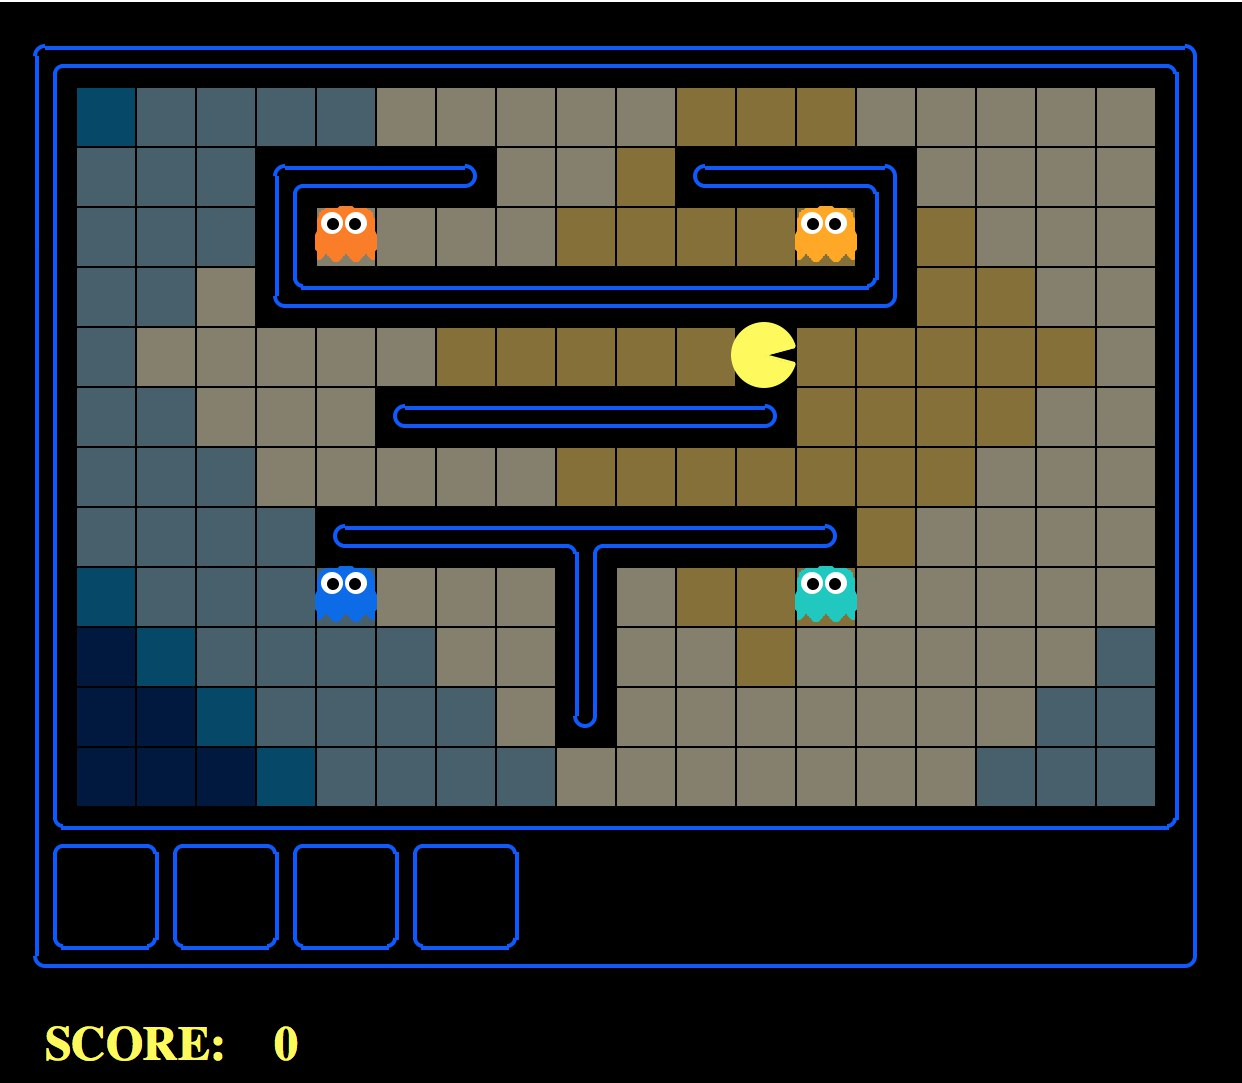
\includegraphics[scale=0.25]{map.jpg}
\end{center}

\newpage
\begin{center}
\subsection{Pregunta 4}

\emph{Analiza el fichero game.py. ¿Qué información ofrece este código sobre el
estado del juego en cada turno? De esta información, ¿cuál crees que podría
ser más útil para decidir automáticamente qué tiene que hacer PacMan?}
\end{center}

En game.py podemos encontrar la clase GameStateData. Esta clase contiene cierta
inforamción sobre el estado del juego, como puede ser la puntuación, si la
partida se ha ganado o perdido, la cantidad de comida que se ha comido, las
capsulas que se han comido, si nueva comida ha sido añadida, e información
sobre el estado de los agentes.

Además, en la clase Agent se pueden ver datos sobre los agentes, tales como su
configuración (posición y dirección), o si el agente es PacMan o un fantasma.

La clase Game contiene referencias a los agentes y a la forma en la que el
juego se muestra en la pantalla, así como el historial de movimientos
realizados.

De la información que se puede encontrar en este archivo, la más relevante para
PacMan podría ser aquella relaccionada con el estado de los agentes (fantasmas),
aunque parte de esta información (por ejemplo, la posición) no está permitida
obtenerla directamente y debe ser inferida a partir de otros parámetros.
Además, la propia dirección y posición de PacMan es también necesaria, tal y
como se ha comentado en la pregunta 2.


\newpage
\begin{center}
\subsection{Pregunta 5}

\emph{Programa una función que imprima en un fichero de texto toda la
información del estado del PacMan. Esta función servirá como una primera
versión de la fase de extracción de características que será imprescindible
en las siguientes prácticas.
\begin{itemize}
    \item Por cada turno de juego, se debe guardar una línea con todos los
    datos concatenados del estado del juego que se calculan por defecto,
    separados por el carácter coma (,).
    \item Además, cada vez que se inicie una nueva partida o se abra el
    juego de nuevo, las nuevas líneas deben guardarse debajo de las antiguas.
    Es decir, que no se debe reiniciar el fichero de texto al empezar una nueva
    partida.
    \item Por tanto, el fichero de texto resultante tendrá que tener tantas
    líneas como turnos se hayan jugado en todas las partidas.
\end{itemize}
}
\end{center}

El objetivo de este apartado era crear una función que sacase a un archivo de
texto inforamción relevante acerca del estado de la partida para que nuestro
agente pueda aprender de estos datos en un futuro. El formato del archivo se
corresponde con una línea por cada turno de la partida en la que los valores
se encuentran separados por una coma.

Para abrir (o crear en el caso de que no exista) un archivo en Python y añadir
nuevas líneas sin borrar las ya existentes, debemos hacerlo de la siguiente
manera:

\centerline{\texttt{f = open('filename', 'a+')}}

Estos son los datos que sacamos, separados por comas, en este orden:
\begin{itemize}
    \item \textbf{Fantasmas que están vivos}: Se representan por booleanos,
    siendo True, que el fantasma que se encuentra en la posición i está vivo, y
    False, no. El primer dato se corresponde con un placeholder para PacMan
    cuyo valor será siempre False.
    \item \textbf{Distancia de PacMan a cada uno de los fantasmas}: Esta
    distancia contendrá cierto ruido y no será del todo precisa.
    \item \textbf{Puntuación de la partida}: La puntuación de la partida en
    cada turno se obtiene por si en un futuro el objetivo de la práctica es
    maximizar este valor.
    \item \textbf{Posición de PacMan}: Obtenemos la posición de PacMan para
    saber en qué lugar del mapa nos encontramos.
    \item \textbf{Dirección de PacMan}: La dirección de PacMan también se
    obtiene para saber hacia dónde nos estamos moviendo (indica la última
    acción tomada).
    \item Además, los últimos datos recogidos se corresponden con 8 valores
    booleanos, los cuatro primeros indican si alguna de las \textbf{celdas
    adyacentes} a las que PacMan podría moverse se corresponden con un
    movimiento ilegal (muro o límite del mapa) y, los otros cuatro, si alguna
    de estas cuatro celdas contiene comida.
\end{itemize}


\newpage
\begin{center}
\subsection{Pregunta 6}

\emph{Implementa manualmente un comportamiento para el PacMan. Para ello se
debe modificar la clase del agente GreedyBustersAgent que se encuentra dentro
del fichero bustersAgents.py. Esta clase es sólo una plantilla que sirve como
punto de partida. PacMan debe perseguir y comerse a todos los fantasmas de la
pantalla.}
\end{center}

En esta sección, comenzamos implementando un agente basándonos en las
indicaciones del código fuente. PacMan elegía como objetivo al fantasma más
cercano fuese cual fuese la posición del resto. Basaba su decisión en la
información dada por un array de Counters \texttt{livingGhostPositionDistributions}
, que contiene pares del tipo (x,y: probabilidad de estar ahí) para cada uno de
los fantasmas. Su funcionamiento era correcto basado en los datos que recibía,
pero estos eran ciegos por lo que el resultado era similar al de un agente
aleatorio.

Tras las aclaraciones posteriores del profesor de prácticas en las que se nos
indicaba que los datos a tener en cuenta no eran los dados por el código sino
la tupla conteniendo las distancias a los fantasmas (atributo de
\texttt{GameState.data}), nos pusimos manos a la obra para diseñar un nuevo
agente basándonos tan sólo en esa información.

Rápidamente descubrimos que la información de un turno aislado no aporta
información alguna, pues si un fantasma está ``a cinco posiciones'', cualquier
acción (norte, sur, este u oeste) tiene a priori las mismas posibilidades de
éxito. De esta forma, tratamos de buscar más información a partir de los mismos
datos.

Llegamos a la conclusión de que, almacenando en dos atributos de nuestro agente
tanto la acción previa como la anterior tupla de distancias podríamos evaluar
en el siguiente movimiento si vamos o no en buena dirección. Esto nos permite
decidir entre dos opciones:

\begin{itemize}
    \item \textbf{Seguir avanzando} (repetir la última acción): si nos estamos
    acercando al objetivo o si éste no se ha alejado (porque, si no se aleja,
    significa que nos movemos en su misma dirección y por tanto la acción
    tomada era la correcta)
    \item \textbf{Cambiar de dirección} (cambiar a una acción aleatoria): si
    nos alejamos o es ilegal seguir avanzando.
\end{itemize}

La elección de seguir avanzando o cambiar de dirección la toma el agente
comparando los \textbf{mínimos} de cada una de las tuplas (actual y previa). De
esta forma, aunque se aleje del fantasma al que perseguíamos, si PacMan se
acerca a otro fantasma y este queda más cerca de él que antes, cambiará de
objetivo automáticamente y seguirá yendo en la misma dirección.

Aunque los movimientos efectuados por este nuevo agente parecen \emph{tener más
sentido} que los del primero cuando le observas jugar mostrando a los fantasmas,
el rendimiento de éste sigue siendo bastante pobre. En nuestro equipo confiamos
en que, si se aplicasen técnicas de aprendizaje automático, se podría mejorar
notablemente la efectividad del agente.

\newpage
\begin{center}
\subsection{Pregunta 7}

\emph{El agente programado en el ejercicio anterior no utiliza ninguna técnica
de aprendizaje automático. ¿Qué ventajas crees que puede tener el aprendizaje
automático para controlar a PacMan?}
\end{center}
Respuesta

\end{document}
